\chapter{À l'abordage du futur}

Si la copie est indispensable à la création et que la société cherche de plus en plus à la punir, sommes-nous condamnés à devoir courir le risque d'un procès à chaque fois que nous créerons quelque chose ?
Je pense que nous pouvons éviter cette situation, et je vais donner des pistes qui vont dans ce sens.

\section{Ne pas devenir esclave du progrès}

Comme je l'ai montré dans la partie \ref*{drm} (page \pageref{drm}), les moyens de contrôle de la copie se sont démocratisés, et avec eux la fonte de certaines de nos libertés fondamentales et d'une partie de notre vie privée.
Mais il n'est pas trop tard pour réagir \dots{}
Avant de poursuivre cette réflexion, je vais devoir expliquer un certain nombre de nouvelles notions.

On commence par la licence d'une œuvre.
Pour faire simple, lorsqu'un créateur produit une œuvre, il peut définir une licence (ou <<~contrat de licence~>>).
Il s'agit un contrat légal qui explique les conditions d'utilisation de l'œuvre, auquel chaque utilisateur doit se plier.

Pour un logiciel, on peut par exemple avoir une licence de type commercial, qui interdit complètement l'utilisation du logiciel sans avoir payé une redevance, ou alors une licence dite <<~freeware~>> qui permet l'utilisation de ce dernier de manière gratuite.

La particularité pour un logiciel est que, dans la plupart des cas, on peut distinguer deux composantes :

\begin{itemize}
\item son code source : c'est ce que le développeur va écrire dans un langage de programmation donné ; il s'agit d'un ensemble de fichiers textes ;
\item son exécutable : il s'agit d'une traduction du code source en langage machine, obtenue par l'action dite de <<~compilation~>> ; l'exécutable est incompréhensible par un humain et on ne peut pas l'utiliser pour récupérer le code source !
\end{itemize}

Pour faire une analogie, disons que le code source est une recette de gâteau ainsi que ses ingrédients, et que l'exécutable est le gâteau lui-même.
Grâce au pâtissier, il est possible d'obtenir un gâteau à partir de sa recette et de ses ingrédients.
Par contre, il ne sera pas possible de récupérer ni la recette ni les ingrédients à partir du gâteau !
On pourra éventuellement récupérer quelques ingrédients qui n'auraient pas été mélangés (comme les petites fraises présentes sur le glaçage) et un bon pâtissier pourra sans doute réécrire une partie de la recette ; mais il ne lui sera pas possible de récupérer tous les ingrédients et la recette exacte !

Certains créateurs distribuent le code source de leur logiciel, on dit alors que le logiciel est <<~libre~>> ou <<~open source~>>.
D'autres ne le font pas et distribuent uniquement l'exécutable.
Leur logiciel est alors dit <<~propriétaire~>> ou <<~privateur~>>.

La notion de logiciel libre a été formalisée en 1983 par Richard Stallman, créateur de la Free Software Foundation\footnote{\url{https://www.fsf.org}}.
La définition d'un logiciel libre est basée sur quatre libertés :

\begin{enumerate}
\item[0.] la liberté d'exécuter le programme, pour tous les usages ;
\item la liberté d'étudier le fonctionnement du programme et de l'adapter à ses besoins ;
\item la liberté de redistribuer des copies du programme (ce qui implique la possibilité aussi bien de donner que de vendre des copies) ;
\item la liberté d'améliorer le programme et de distribuer ces améliorations au public, pour en faire profiter toute la communauté.
\end{enumerate}

Certains logiciels propriétaires peuvent donner les libertés \no{}0 et \no{}2 à l'utilisateur, mais rendent les deux autres libertés inaccessibles puisqu'ils ne distribuent pas leur code source.

Au delà de l'aspect légal, le logiciel libre est une philosophie.
Il s'agit de rendre le contrôle à l'utilisateur : il a les moyens d'étudier le programme qui va s'exécuter sur son matériel, et de le modifier s'il ne lui plait pas.
Cette possibilité de pouvoir étudier le fonctionnement d'un logiciel peut paraitre inutile pour le commun des mortels, qui ne connait pas la programmation, mais c'est pourtant quelque chose de très important !

Plus un logiciel libre a du succès, plus des utilisateurs avancés vont (statistiquement) l'étudier.
Si ce logiciel contient des mécanismes nocifs pour l'utilisateur (DRM, récolte et envoi de données personnelles, etc.) ou des failles de sécurité pouvant nuire à l'utilisateur, alors un signal d'alarme est tiré, et le logiciel incriminé va devoir revoir sa copie ou sera soigneusement évité par la communauté.

Ceci assure que presque l'intégralité des logiciels libres prennent soin de la sécurité et de la vie privée de l'utilisateur.
Les utilisateurs de logiciels propriétaires doivent quant à eux faire confiance aux auteurs du logiciel pour toutes ces questions.
Quand il s'agit de logiciels édités par des entreprises, dont le but est par définition de faire du profit, on peut se demander si c'est bien placer sa confiance \dots{}

La différence entre le libre et l'open source est principalement une différence de philosophie.
Le logiciel libre met en avant la liberté qu'il apporte à ses utilisateurs, tandis que le logiciel open source va apprécier la communauté de développeurs qui va se former autour de lui et lui permettre de se développer plus efficacement.
En pratique, presque tous les logiciels libres correspondent à la définition d'un logiciel open source et inversement.

Pour ne pas avoir à réécrire à chaque fois un nouveau contrat de licence pour leurs nouvelles créations, les développeurs de logiciels libres ont tendance à récupérer des textes de licences existantes (qui la plupart du temps sont libres eux aussi).
Certaines licences sont donc très répandues parmi les logiciels libres.
On peut citer, par exemple, la GNU General Public License\footnote{Écrite par Richard Stallman lui-même, pour son projet GNU} (GNU GPL) ou la licence MIT\footnote{Du nom de l'université qui l'a créée (Massachusetts Institute of Technology)}.

La licence MIT donne à toute personne recevant le logiciel le droit illimité de l'utiliser, le copier, le modifier, le fusionner, le publier, le distribuer, le vendre et de changer sa licence, à la seule condition que les noms des auteurs soient cités, même en cas de modification du logiciel.
La licence GNU GPL offre des droits similaires, à la différence qu'elle met en œuvre la notion de copyleft\footnote{Il s'agit d'un jeu de mot basé sur le mot <<~copyright~>> ; l'idée de copyleft est opposée à celle de copyright}, ce qui veut dire que le logiciel doit être redistribué avec la même licence, même s'il a été modifié.

\begin{quotation}
\textit{<<~L'idée centrale du copyleft est de donner à quiconque la permission d'exécuter le programme, de le copier, de le modifier, et d'en distribuer des versions modifiées - mais pas la permission d'ajouter des restrictions de son cru. C'est ainsi que les libertés cruciales qui définissent le logiciel libre sont garanties pour quiconque en possède une copie ; elles deviennent des droits inaliénables.~>>}
\begin{flushright}Richard Stallman\end{flushright}
\end{quotation}

Les logiciels libres permettent donc de ne pas devenir esclaves du progrès, car ils donnent le pouvoir aux utilisateurs, et non pas à leurs créateurs comme c'est le cas pour les logiciels propriétaires.
Les logiciels sont déjà partout, pas seulement dans nos ordinateurs, et il nous revient de choisir si nous voulons garder le contrôle sur notre technologie, ou le confier à des sociétés dont le but est de faire du profit.

Il est facile de faire ressentir ce besoin du logiciel libre contre l'esclavage grâce au domaine médical\footnote{Un autre exemple que celui que je vais développer ici est disponible à cette adresse : \url{http://www.framablog.org/index.php/post/2012/11/26/un-coeur-gros-comme-ca}}.
Il existe actuellement un bon nombre d'appareils médicaux dont le fonctionnement est régit par des logiciels (par exemple, les stimulateurs cardiaques, ou <<~pacemakers~>>).
On peut dire que ces appareils ne valent que ce que valent leurs logiciels.
Si ces logiciels sont propriétaires, il n'est pas rassurant de se dire qu'on a dans le corps des appareils dont le comportement n'est connu que par la société qui les a fabriqués.

S'ils étaient libres, ils pourraient à coup sûr bénéficier de nombreuses relectures par des experts d'horizons différents, ce qui réduirait le nombre de bogues\footnote{Francisation de l'anglais <<~bug~>> qui désigne un défaut de conception d'un programme informatique à l'origine d'un dysfonctionnement}.
Car oui, les logiciels ont des bogues.
Et lorsque ces logiciels nous maintiennent en vie, un bogue peut être fatal.
Et avec un code fermé, qu'est ce qui empêche l'appareil d'envoyer nos signaux vitaux en sans-fil à notre insu ?
Ou, s'il est nécessaire que ces informations soient envoyés en sans-fil à un autre appareil, la connexion sans-fil est-elle correctement sécurisée ?
Si ce n'est pas le cas, peut être que quelqu'un peut communiquer avec notre pacemaker et lui donner l'ordre de s'arrêter \dots{}

Le logiciel libre est un bouclier contre ce genre de pratiques et de négligences, et, en ce sens, il est indispensable.

Je vais terminer cette partie sur un dernier point : celui du patrimoine.
J'ai dit, lorsque j'ai expliqué le droit d'auteur (page \pageref{droit-auteur}), que lorsqu'on crée une œuvre de l'esprit, on se voit alors automatiquement doté de droits exclusifs relatifs à l'exploitation de cette œuvre.
Contrairement au système des brevets, qui n'offre pas de droits automatiques, le système du droit d'auteur (et du copyright) ne possède pas de base de données indiquant pour chaque œuvre son auteur, ainsi que les droits d'exploitation que celui-ci a cédé (ou pas) et à qui.

\label{oeuvres-orphelines}
Il se pose alors le problème d'œuvres orphelines, c'est à dire n'ayant pas d'auteur connu.
On ne peut actuellement pas considérer que ces œuvres font partie du domaine public, et pour cette raison, leur utilisation est un risque.

Par exemple, on peut imaginer que, voulant utiliser une œuvre dans un de mes projets, je décide de contacter son auteur pour négocier la permission d'intégrer tout ou partie de son travail dans le mien.
Ne parvenant pas à trouver cet auteur, je décide tout de même d'utiliser l'œuvre.
Quelques années plus tard, l'auteur en question réapparait, prouve qu'il est bien l'auteur de l'œuvre que j'ai utilisée, et me fait un procès pour violation du droit d'auteur.
Je perds et je dois lui payer une énorme amende.

Conclusion : une œuvre orpheline est <<~bloquée~>> entre la zone de droit et le domaine public, et l'utiliser comporte le même risque que celui d'utiliser une œuvre protégée sans l'autorisation de son 	auteur.

J'en parle ici car, pour moi, si nous ne voulons pas que les générations futures deviennent esclaves de la technologie et des idées contrôlées par une minorité, nous devons lui donner les moyens de les apprivoiser.
Et cela passe par la possibilité de ce servir des œuvres et des idées que nous allons leur léguer.
Malheureusement, le système actuel ne semble pas aller dans ce sens ; il ne tient qu'à nous de le faire évoluer, mais j'y reviendrai plus tard \dots{}

%(logiciel libre, donner le pouvoir aux utilisateurs, assurer le patrimoine, exemple du domaine médical)
\section{Partager pour mieux créer}

Comme nous l'avons vu précédemment, lorsqu'on crée, on s'inspire d'œuvres existantes, voire on les réutilise (partiellement ou intégralement).
Empêcher ce processus revient à entraver la créativité.
Mais, au contraire, le favoriser peut conduire à une créativité sans limite !

Pour cela, il faut redéfinir les lois sur la protection du droit d'auteur, mais nous en reparlerons.
L'autre possibilité est que les créateurs autorisent les autres à exploiter leurs œuvres.

On pourrait se dire que ces créateurs doivent manger, et ont donc besoin de vendre leurs œuvres.
C'est peut être vrai pour une économie de la rareté, mais, si on parle d'œuvres de l'esprit, les règles du jeu sont totalement différentes.
Il existe de nombreuses entreprises qui réussissent à vivre en publiant leur travail sous licence libre.
C'est notamment le cas de Red Hat, une société américaine éditrice de distributions Linux, qui a obtenu un chiffre d'affaire de 1 milliard de dollars américains en 2012.

Énormément de produits que nous connaissons sont basés sur des logiciels libres.
Cela veut dire que si les créateurs de ces logiciels n'avaient pas rendu libres leurs créations, aucun produit n'aurait pu se baser dessus et il aurait fallu réinventer la roue à chaque fois.

Par exemple, ma Freebox Révolution\footnote{Modem ADSL amélioré du fournisseur d'accès à Internet <<~Free~>>} embarque pas moins de 67 logiciels libres\footnote{D'après la page <<~Mentions légales~>> dans la console d'administration de la Freebox Révolution}.
Si ces logiciels n'avaient pas été libres, les développeurs de chez Free auraient du en écrire des nouveaux qui réalisaient les mêmes fonctions.
La Freebox n'aurait pas été rentable pour Free, et ne serait peut être même jamais sortie.

On peut aussi constater que Free a parfois amélioré certains de ces logiciels, probablement pour corriger quelques imperfections ou ajouter une fonction dont ils avaient besoin pour leur Freebox.
Ces modifications ont soit été publiées elles-mêmes sous licence libre, soit directement poussées vers les créateurs des logiciels concernés, dans le but que ceux-ci les intègrent à terme et en fassent bénéficier la communauté.

Cet échange de bons procédés (<<~j'utilise ton programme et en échange je partage avec toi et ta communauté les éventuelles améliorations que je lui apporterais~>>) est très courant dans le monde du libre et de l'open source.
Il ne s'agit pourtant pas d'une obligation légale : rien de tel n'est inscrit dans les contrats de licence des logiciels en question.
Il s'agit tout bonnement de créativité engendrée par le partage, et cela permet un progrès pour tous.

On peut aussi évoquer tout ce qui touche à la philosophie des hackers.
Contrairement à ce que les médias peuvent dire, le terme <<~hacker~>> n'est pas négatif.
<<~Un hacker est quelqu'un qui aime comprendre le fonctionnement d'un mécanisme, afin de pouvoir le bidouiller pour le détourner de son fonctionnement originel.~>>\footnote{Source : \url{https://fr.wikipedia.org/wiki/Hacker}}

Le hacking est une forme de créativité encore peu connue du commun des mortels.
Pourtant, de nombreuses avancées technologiques sont attribuées à des hommes qu'on pourrait qualifier de hackers.
Parfois, la curiosité pousse à aller étudier le fonctionnement d'un système donné (appareil, logiciel, voire même l'art !).
Et parfois, cette étude donne de nouvelles idées auxquelles le créateur original n'avait pas initialement pensé.
Cette approche décalée permet d'identifier des failles potentielles de sécurité qui n'auraient jamais été imaginées avec une approche <<~classique~>> de test.

Par exemple, dans les années 60, John Draper découvre un sifflet dans sa boite de céréales Cap'n Crunch.
Il se rend ensuite compte que ce sifflet est accordé sur le <<~la aigu~>>, et lui permet de reproduire la tonalité à 2600 Hz utilisée par la compagnie téléphonique Bell pour ses lignes longue distance.
Pour faire simple\footnote{Les détails sont disponibles ici : \url{https://fr.wikipedia.org/wiki/John_Draper} (et sur bien d'autres sites)}, ce sifflet lui permet de passer des appels internationaux gratuitement, grâce à une faille dans le système téléphonique.
Il fera deux mois de prison et gardera le surnom <<~Captain Crunch~>>.
Ce genre d'anecdote est amusant, mais plus courant qu'on le croit.

Il faut favoriser ces démarches de hackers car elle ont une portée éducative, d'autant plus que l'histoire montre que c'est souvent le point de départ de nombreux progrès.
Et tout cela se met en place autour de logiques de partage.

Le phénomène <<~d'aversion à la perte~>> est une composante de la psychologie humaine.
Il fait référence à la tendance d'une personne à préférer éviter des pertes plutôt que d'acquérir des gains.
Dans notre étude, c'est, j'en suis convaincu, l'un des facteurs qui empêchent les créateurs de partager leurs œuvres.
De nombreux cas ont montré qu'il y avait souvent beaucoup plus à retirer du libre partage des œuvres que la <<~perte~>> du contrôle de ces œuvres.
Ce qui est arrivé au musicien Andy Othling illustre bien cette idée\footnote{Voir : \url{http://www.framablog.org/index.php/post/2012/10/30/ma-musique-gratuite-pendant-24h}}.

On pourrait également parler plus longuement du domaine de la mode.
Il n'y a en effet pas de copyright dans cette industrie, et pourtant elle est très rentable.
On peut même dire que c'est ce qui pousse les stylistes à créer toujours plus, sans avoir à craindre un procès parce qu'ils ont réutilisé une idée d'un concurrent.
Je ne m'étendrais pas là dessus, dans la mesure où la conférence TED animée par Johanna Blakley\footnote{\url{http://www.ted.com/talks/johanna_blakley_lessons_from_fashion_s_free_culture.html}} le fait très bien.

L'histoire montre, comme le rappelait Henry Ford (voir la citation page \pageref{ford}), que lorsque tous les facteurs qui rendent le progrès possible sont là, celui-ci devient inévitable.
On peut citer comme exemple le téléphone : le brevet concernant le téléphone fut déposé à deux heures d'intervalle par Alexander Graham Bell et Elisha Gray !
Partager, c'est s'assurer que les facteurs qui rendent le progrès possible soient là.
Nous avons besoin d'un progrès inévitable.

%(partager le plus possible, aller contre l'aversion à la perte, hacker, exemple du téléphone, exemples de réussites du libre, exemple de Arduino, exemple de la mode)
\section{Valoriser les créateurs}

Je parlais précédemment de l'affaire Megaupload.
Megaupload était un service de stockage de données dans le cloud.
Il était connu en grande partie pour sa capacité de pouvoir être utilisé comme plateforme de partage.
En effet, un utilisateur pouvait partager un lien qui permettait aux autres utilisateurs de récupérer une copie du fichier concerné.
Megaupload était donc très gênant pour les ayants droit, car il permettait aux gens de s'échanger librement des créations normalement payantes.
Cela représentait, selon eux, un manque à gagner énorme.

En janvier 2012, le FBI fait fermer Megaupload, ou plutôt il saisit les serveurs de ce dernier qui étaient situés dans l'État de Virginie, aux États-unis.
Bien évidemment, sans ses serveurs Megaupload est inaccessible et les utilisateurs n'ont plus accès à leurs données.
Je ne reviendrai pas sur la légitimité de cette saisie, celle ci ayant été ordonnée de manière très douteuse.

Ce qui m'intéresse ici c'est l'étude qui a été publiée récemment par la Munich School of Management et la Copenhagen Business School\footnote{Source : \url{http://ssrn.com/abstract=2176246}}.
Ces chercheurs allemands et norvégiens ont analysé les données hebdomadaire des cinémas dans 49 pays, de 2007 à 2012.
La conclusion est la suivante : << La fermeture de Megaupload a eu un effet négatif sur les recettes du box-office, hormis dans certains cas où l'effet été négligeable~>>.

Selon eux, Megaupload présentait un <<~effet de réseau (social) où le partage de fichiers agit comme un mécanisme pour diffuser des informations venant de personnes qui ont une volonté faible ou nulle de payer, envers des personnes qui ont une grande volonté de payer~>>.
Toujours selon eux, le cinéma d'auteur a été bien plus touché par cette fermeture que les blockbusters américains, car bénéficie d'une très faible promotion auprès des médias, et donc compte beaucoup plus sur le bouche-à-oreille.

Dans la même catégorie, l'OFCOM, l'autorité de régulation des télécoms du Royaume-Uni, a publié cette semaine une étude\footnote{Source :\\\url{http://www.pcinpact.com/news/75538-la-consommation-pirates-britanniques-sous-oeil-dune-etude.htm}}, menée auprès de 4 400 britanniques âgés de plus de 12 ans par le cabinet Kantar Media.

À partie de cette étude, le site \href{http://torrentfreak.com/uk-movie-pirates-spend-way-more-at-the-box-office-121122/}{TorrentFreak} a établi trois catégories d'internautes : ceux qui ont uniquement eu recours à des moyens illégaux pour profiter d'œuvres protégées, ceux n'ayant opté au contraire que pour des solutions légales, et une troisième population, qualifiée d'hybride car regroupant les internautes ayant pratiqué les deux. Ils ont ensuite transposé les sommes qu'ont déclaré avoir dépensé ces individus en biens culturels (cinéma, musique, télévision).

\begin{figure}[H]
\center
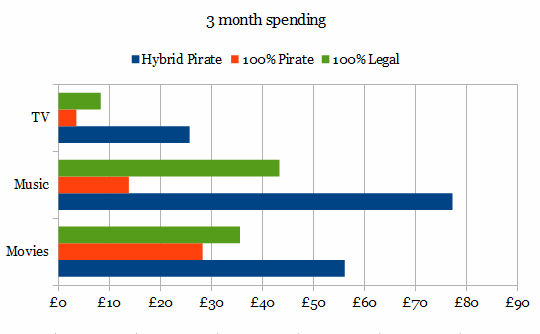
\includegraphics[scale=.893]{images/budget-culture.png}
{\footnotesize Source : \url{http://torrentfreak.com/uk-movie-pirates-spend-way-more-at-the-box-office-121122/}}
\caption{Budget culture/divertissement des internautes anglais}
\end{figure}

On remarque que ce sont à chaque fois les internautes <<~hybrides~>> qui vont le plus dépenser, et non pas, comme on pourrait le croire, ceux qui empruntent uniquement le chemin de la légalité.

Ces deux études convergent vers une conclusion similaire : le libre partage des œuvres ne tue pas la création, au contraire.

Il faut voir que les nouvelles technologies numériques ont rendu quasiment obsolètes les industries de la culture.
Ce sont déjà qui sont déjà arrivées, et qui arriveront encore.
Laissez-moi vous parler des vendeurs de glace \dots{}\footnote{Source : \url{http://reformedroitauteur.sploing.fr/\#htoc93}}

Il y a 100 ans, la compagnie <<~Stockholm Is~>> était l'un des plus importants employeurs de Stockholm en Suède. Leur commerce était aussi simple que nécessaire : aider à conserver les denrées périssables plus longtemps en distribuant du <<~froid~>> dans un format adéquat.

Pour cela, ils découpaient durant l'hiver de grands blocs de glace sur les lacs gelés, les conservaient dans des granges sur de la sciure, coupaient les blocs en de plus petits morceaux et les revendaient dans la rue. Les gens achetaient alors la glace et l'entreposaient avec la nourriture dans des placards spéciaux, les aliments étaient ainsi conservés au frais.

Lorsque durant la première moitié du siècle dernier les foyers de Stockholm furent équipés de l'électricité, ces revendeurs de froid devinrent obsolètes. Après tout, ce qu'ils proposaient n'était rien d'autre que la possibilité de conserver la nourriture au frais, et à présent tout le monde en était capable.

Ce fut un processus assez rapide dans les villes. Avec la disponibilité du réfrigérateur à partir de 1920 environ, la plupart des foyers acquirent le leur à la fin des années trente. L'un des plus importants employeurs de la ville devint complètement obsolète à cause d'une avancée technique.

Il y eu de nombreuses tragédies personnelles à cette époque du fait que les vendeurs de glace perdirent leur gagne pain et durent se former afin de retrouver un emploi dans un nouveau secteur. Les vendeurs de glace ont souvent eu du mal à se reconvertir, et voir leur secteur se désintégrer à toute vitesse ne les a pas aidé.

Voici quelques faits qui n'ont pas eu lieu lorsque l'industrie de distribution de glace devint obsolète :

\begin{itemize}
\item Aucun propriétaire de réfrigérateur ne fut poursuivi en justice pour <<~production de son propre froid~>>, ignorant ainsi les sociétés de distribution de froid.
\item Aucune loi ne fut proposée pour rendre les compagnies d'électricité passibles de poursuites dans le cas où l'électricité qu'elles fournissaient aurait été utilisée d'une manière pouvant porter préjudice au travail de vendeur de glace.
\item Personne ne demanda une taxe mensuelle aux propriétaires de réfrigérateur au profit du syndicat des vendeurs de glace.
\item Il n'y a pas eu de prolifération de coûteux panels d'experts pour soutenir combien les vendeurs de glace étaient importants pour l'économie toute entière.
\end{itemize}

\textit{Oui, ce sont des choses qui sont arrivées de nos jours \dots{}}

Par contre, la distribution monopolistique devint obsolète et l'économie en général bénéficia de cette décentralisation.

On apprend de l'histoire, qu'à chaque fois qu'une industrie devient obsolète, cela est bénéfique.
Cela traduit que l'on a appris quelque chose d'important : faire les choses d'une manière plus efficace.
De nouvelles compétences et de nouveaux secteurs industriels apparaissent toujours dans leurs sillages.

Les industries actuelles devraient s'adapter au progrès, et pas tenter d'adapter le progrès à leurs modèles économiques vieillissants.
Je pense que nous sommes à l'aube d'une révolution : celle de l'industrie de la culture et de la question du partage des œuvres de l'esprit.

Il faut réinventer des modèles économiques qui profitent aux créateurs et à ceux qui ajoutent de la valeur.
C'est encore une fois une problématique complexe, d'autant que, cette fois ci, il faut penser ces modèles dans une logique d'abondance et non plus de rareté.
Certaines idées ont déjà émergé, mais toutes ne sont pas bonnes.
L'exemple qui va suivre est très inspiré du chapitre 6 du document <<~Sur la réforme du droit d'auteur~>>\footnote{\url{http://reformedroitauteur.sploing.fr/}}.

La licence globale, par exemple, est un forfait illimité pour la culture sous forme d'une taxe sur l'Internet haut débit.
C'est une idée qui est dans l'air du temps depuis au moins une décennie, mais n'est jamais devenue réalité.
L'idée semble simple et éventuellement attractive au premier abord, mais lorsque l'on commence à s'intéresser aux détails afin de formuler une proposition concrète, on prend conscience des problèmes.

Collecter l'argent est une chose. On peut discuter pour savoir si c'est juste d'obliger les gens qui ne téléchargent rien à payer quand même, ou pour savoir pourquoi des entreprises devraient être dédommagées pour cause de progrès technologique, ou encore pour savoir comment prendre en compte les multiples connexions à Internet que possède une famille.
Mais laissons cela de côté.
C'est lorsque l'on se demande comment l'argent devrait être réparti que les choses amusantes commencent.

Si l'on calcule les gains des artistes sur base de ce qui est joué à la télévision et la radio, la plupart de l'argent va aller aux artistes établis qui gagnent déjà très bien leur vie.
C'est la manière dont fonctionne le système actuellement avec les prélèvements sur les supports vierges et les appareils électroniques.
L'une des caractéristiques les plus intéressantes d'Internet, c'est le fait que les plus petites performances confidentielles peuvent atteindre leur public, même si elles ne sont pas jouées à la télévision et la radio. L'addition de toutes les petites performances constitue une part importante de ce qui est téléchargé sur le net.

Ces petits artistes sont ceux que la plupart des gens souhaitent supporter, à la fois pour la diversité culturelle qu'ils assurent, et simplement parce que très souvent ils ont vraiment besoin de ces revenus.
Avec un forfait basé sur la diffusion à la télévision et la radio, ils n'obtiendraient qu'une très faible partie de l'argent collecté.
Dans le même temps, leurs aficionados disposeraient de moins de ressources financières pour supporter ces artistes, puisqu'ils auront déjà dû payer le forfait.
L'effet immédiat serait un système qui diminue les revenus des artistes pauvres et distribue l'argent à ceux qui sont déjà riches.

Une alternative, préférée par le plus grand nombre des partisans de la licence globale, est au contraire de mesurer ce qui est partagé sur internet et de baser les gains aux artistes sur ces mesures. Mais cela engendre d'autres problèmes.

35\% des téléchargements sur Internet sont de la pornographie\footnote{Source : \url{http://www.numerama.com/magazine/16005-la-pornographie-occupe-un-tiers-du-web-selon-\\une-societe-specialisee-dans-le-filtrage.html}}.
L'industrie pornographique possède exactement la même protection du droit d'auteur que les autres productions audiovisuelles.
Si les paiements d'un forfait culturel sont considérés comme un <<~dédommagement~>> pour le téléchargement d'œuvres protégées par le droit d'auteur, alors 35\% de l'argent devrait immédiatement reversé à l'industrie pornographique.

Le point ici n'est pas de critiquer la pornographie en tant que telle.
Mais ça ne veut pas dire qu'il ait besoin de milliards provenant de subventions gouvernementales.
Au cours de l'histoire, c'est une industrie qui a démontré sa capacité à s'adapter de son propre chef.

Si on veut exclure la pornographie, on ne pourra plus dire que la licence globale rémunère les artistes qui sont appréciés, ou alors il faudra inventer une organisation qui aurait pour but de décréter où se situe la limite entre art et pornographie \dots{}

Il est techniquement possible de mesurer ce qui est partagé sur Internet avec une précision relativement élevée.
Mais à la minute à laquelle on commencera à rémunérer suivant des statistiques de téléchargement, les gens changeront de comportement.
Aujourd'hui, si vous aimez un artiste qui a produit un nouvel album, vous le téléchargez pour pouvoir l'écouter.
Mais si vous savez que votre artiste préféré gagnera de l'argent en proportion de vos téléchargements, vous le retéléchargerez sans cesse pour l'aider.
Ainsi, Internet sera en permanence congestionné par du trafic inutile, peu importe la capacité ajoutée par les opérateurs.

Les virus sont aujourd'hui un problème majeur, malgré qu'il soit assez difficile pour leurs créateurs de les rentabiliser.
Le but d'un virus est généralement d'installer une porte dérobée dans votre ordinateur, pour que celui-ce devienne part d'un réseau d'ordinateurs vérolés, un botnet, que le créateur du virus peut contrôler à sa guise.
Le détenteur d'un botnet peut vendre ses services à des organisations criminelles qui veulent envoyer du spam ou commettre diverses formes de fraude, mais à moins qu'il ait des liens avec le crime organisé, il n'est pas facile pour lui de rentabiliser ses talents.
Avec une licence globale, tout change.

Chaque propriétaire d'un botnet n'aurait plus besoin que d'avoir un ami qui a enregistré une chanson couverte par le droit d'auteur.
Ses milliers d'ordinateurs sous contrôle n'auront qu'à télécharger sans répit cette chanson.
Grâce à la licence globale, ces téléchargements généreront automatiquement des revenus pour son ami.
Pour les formes de fraude les plus simples, la police arrivera peut-être à détecter son activité criminelle et à y mettre fin, mais on peut facilement imaginer que des systèmes de fraude sophistiqués verront le jour.
La licence globale deviendrait donc une excellente source de revenu pour les criminels, pour les éditeurs de virus.

La licence globale n'est donc pas une solution viable.
Mais surtout, elle répond à des problèmes qui n'existent pas !

Internet est une technologie révolutionnaire qui change la plupart des présuppositions de l'industrie de la culture.
La tâche des politiques n'est pas de protéger les vieux modèles économiques ou d'en inventer de nouveaux.
Ils doivent seulement s'assurer que la société dans laquelle nous vivons puisse être florissante et que les gens créatifs peuvent gagner leur vie avec ce qu'ils font.

C'est pour cette raison que j'affirme : il faut valoriser les créateurs.

%(les pirates achètent, inutilité licence globale, inventer des modèles économiques, exemple des vendeurs de glace)
\section{La réforme du système actuel}

On assiste donc à une véritable lutte des pouvoirs.
Les industries de la culture sont en train d'essayer de freiner le progrès pour engendrer plus de profit.
Elles n'hésitent pas à faire du lobbying auprès de nos politiques qui semblent, pour la plupart, dépassés par ces problématiques.

Heureusement, il existe un parti politique qui traite ces problèmes et qui commence doucement à s'implanter en Europe et dans le monde entier : le Parti pirate.

Le Parti pirate s'attache notamment à réformer les droits de la propriété intellectuelle et à soutenir ou renforcer les droits fondamentaux relatifs à la vie privée.
Le programme du parti se concentre sur ce sujet transversal et il n'est donc pas possible d'attribuer au Parti pirate une position de droite ou de gauche.

Ce parti est un phénomène mondial : il existe des Partis pirates dans de nombreux pays à travers le monde.
Ceux-ci sont des entités indépendantes les unes des autres, mais sont reliés par le Parti pirate international.

À l'origine, le premier Parti pirate fut créé en Suède, mais le mouvement a également été représenté lors d'élections en Allemagne et en France\footnote{Voir leur site : \url{http://www.partipirate.org/}}.

Voici donc les réformes du droit d'auteur que propose le Parti pirate.

\paragraph{Mesure 1}
\textit{Personne ne devrait être autorisé à déclarer qu'il est Paul Mc Cartney s'il ne l'est pas.
Ce devrait être illégal.
<<~Rendre à César ce qui est à César >> est une maxime qui met tout le monde d'accord.}

Dans les faits, c'est un concept qui est très bien appliqué sur Internet.
Les blogueurs ont tendance à citer leurs sources d'une façon qui fait bien plus que respecter le minimum légal.
Il y a plusieurs raisons à cela.
Cela rend leur blogue plus crédible s'ils donnent les liens vers leurs sources afin que leurs lecteurs puissent en vérifier l'origine s'ils le souhaitent.
Les personnes qu'ils citent sont contentes, elles seront donc plus enclines à citer les blogues en question si l'occasion s'y présente, et ceux-ci verront leur trafic augmenter.
Voilà les raisons pratiques pour lesquelles il est dans l'intérêt d'un blogueur d'être plus généreux au niveau des citations de ses sources que ne l'exige aucune loi.

Le droit d'être reconnu en tant qu'auteur sur Internet n'est pas menacé.
Le Parti pirate propose donc de laisser inchangé ce point de la législation du droit d'auteur.

\paragraph{Mesure 2}
\textit{Nous voulons que le droit d'auteur redevienne ce pourquoi il a été conçu, et rendre clair qu'il ne doit réguler que les échanges commerciaux. Copier ou utiliser un travail protégé sans but lucratif ne devrait jamais être interdit.
Le pair à pair est, entre autres, une bonne raison pour cette légalisation.}

Pour eux, une telle avancée est :

\begin{itemize}
\item inéluctable : la limitation du partage de fichiers par les lois et la répression ne fonctionnent pas, et sont contournées.
\item indispensable : les tentatives d'imposer l'interdiction du partage de fichiers mettent en danger les droits fondamentaux.
\item inoffensive : les artistes et le secteur de la culture, dans leur ensemble, se portent bien malgré le partage de fichiers (ou peut être grâce à lui), il n'y a donc pas de réel problème à résoudre.
\item facile à mettre en place : <<~Suivre l'argent~>> suffit aux autorités pour leur permettre de garder une trace des activités commerciales.
\end{itemize}

\paragraph{Mesure 3}
\textit{Nous souhaitons raccourcir les durées de protection à quelque chose de raisonnable à la fois du point de vue de la société et des investisseurs, et nous proposons 20 années à partir de la publication.
Nous souhaitons la même période de protection pour tous les types de création.}

On pourrait se dire qu'il serait intéressant d'adapter la durée de la protection au type d'œuvre auquel on a affaire.
Malheureusement il s'avère en pratique difficile de trouver un compromis, les avis divergeant énormément en fonction des sensibilités de chacun.

De plus, dans la plupart des projets culturels sérieux, on attend que le projet s'autofinance et commence à dégager des bénéfices au bout de quelques années, grand maximum.
Ces projets n'ont pas besoin d'une protection de la durée d'une vie, étant donné qu'ils sont prévus par les investisseurs pour être rentabilisés en quelques années.

\paragraph{Mesure 4}
\textit{La protection du droit d'auteur devrait être accordée automatiquement dès la publication comme aujourd'hui, mais si les propriétaires veulent continuer à jouir de leurs droits après les cinq premières années de publication, ils devraient se manifester de sorte qu'ils soient facilement trouvables.}

J'en parlais précédemment (page \pageref{oeuvres-orphelines}), le problème des œuvres orphelines est bien réel.
Environ 75\% des livres que Google souhaite numériser dans le cadre de leur <<~Google Books initiative~>> sont épuisés, mais toujours sous droits d'auteur.
Même s'il est théoriquement possible de retrouver le détenteur des droits pour beaucoup de ces livres en entreprenant une investigation pour chaque cas individuel, cela devient en pratique infaisable lorsqu'on veut numériser en masse.

Ce que propose le Parti pirate, c'est que si on désire une rémunération pour l'usage d'une de nos œuvres plus vieille que 5 ans, on doit faire savoir auprès d'une base de données publique comment être contacté et où faire parvenir l'argent.

\paragraph{Mesure 5}
\textit{Nous voulons changer la situation en introduisant des exceptions claires de droit au remix ou à la parodie, de même que de droits de citation pour les matériaux audiovisuels qui se calquent sur la législation existante pour les textes.}

Peut on être propriétaire d'un son ? 
Aujourd'hui, la réponse à cette dernière question est malheureusement oui.
Les majors revendiquent la propriété sur des sons individuels et de très courts extraits.
Si on est un musicien hip-hop, il faut s'attendre à payer des centaines de milliers d'euros par avance pour avoir le droit d'utiliser des samples si on souhaite toujours rendre sa musique accessible au public \dots{}

C'est clairement une restriction du droit de créer de nouvelles cultures.

\paragraph{Mesure 6}
\textit{Il devrait être systématiquement légal de passer outre les MTP\footnote{MTP = DRM ; j'en parle page \pageref{drm}} et nous devrions bannir les MTP qui empêchent des usages légaux.
Les grandes multinationales ne devraient pas avoir le droit d'écrire leurs propres lois d'utilisation des fichiers.}

J'ai déjà évoqué ce thème, assez largement je pense pour convaincre de sa nocivité pour la création.

\vspace{50pt}

Il faut garder en tête que si ces réformes constituent un objectif, la plus difficile sera de trouvera le meilleur chemin pour y arriver.
J'espère vraiment que les bonnes personnes seront mises au pouvoir bientôt, car il est urgent de réformer le droit d'auteur.
Aucun modèle économique ne vaut mieux que nos droits civiques.

% état final != transition
%(lutte de pouvoirs, propositions du parti pirate)
